\section{异构数据并行计算}

数据并行是指对数据集的不同部分执行的计算工作可以彼此独立地完成,从而可以彼此并行地完成的现象。 
许多应用程序表现出丰富的数据并行性,这使得它们适合可扩展的并行执行。 
因此,并行程序员熟悉数据并行性的概念以及编写利用数据并行性的代码的并行编程语言结构非常重要。 
在本章中,我们将使用 CUDA C 语言结构来开发一个简单的数据并行程序。

\subsection{数据并行}
当现代软件应用程序运行缓慢时,问题通常是数据——数据太多而无法处理。 
图像处理应用程序处理具有数百万到数万亿像素的图像或视频。 科学应用程序使用数十亿个网格点对流体动力学进行建模。 
分子动力学应用必须模拟数千到数十亿个原子之间的相互作用。 航空公司的调度涉及数千个航班、机组人员和机场登机口。 
大多数像素、粒子、网格点、交互、飞行等通常可以在很大程度上独立处理。 例如,在图像处理中,
将彩色像素转换为灰度仅需要该像素的数据。 模糊图像会平均每个像素的颜色与附近像素的颜色,仅需要该小像素邻域的数据。 
即使是看似全局的操作,例如查找图像中所有像素的平均亮度,也可以分解为许多可以独立执行的较小计算。 
这种对不同数据块的独立评估是数据并行性的基础。 编写数据并行代码需要(重新)组织围绕数据的计算,
以便我们可以并行执行最终的独立计算,从而更快地完成整个工作——通常要快得多。
\begin{figure}[H]
	\centering
	
\includegraphics[width=0.9\textwidth]{figs/F2.1.png}
	\caption{\textit{将彩色图像转换为灰度图像。}}
\end{figure}

让我们通过一个彩色到灰度转换的例子来说明数据并行的概念。 图 2.1 显示了由许多像素组成的彩色图像(左侧),
每个像素包含从 0(黑色)到 1(全强度)变化的红色、绿色和蓝色分数值(r、g、b)。

为了将彩色图像(图 2.1 左侧)转换为灰度图像(右侧),我们通过应用以下加权和公式计算每个像素的亮度值 L:
\begin{equation*}
	L = r*0.21 + g*0.72 + b * 0.07
\end{equation*}

\begin{remark}[RGB 彩色图像表示]
在 RGB 表示中,图像中的每个像素都存储为 (r, g, b) 值的元组。 
图像行的格式为 (r g b) (r g b) ... (r g b),如下面的概念图所示。 
每个元组指定红色 (R)、绿色 (G) 和蓝色 (B) 的混合。 也就是说,
对于每个像素,r、g、b 值代表渲染该像素时红、绿、蓝光源的强度(0 为暗,1 为全强度)。
\begin{figure}[H]
	\centering
	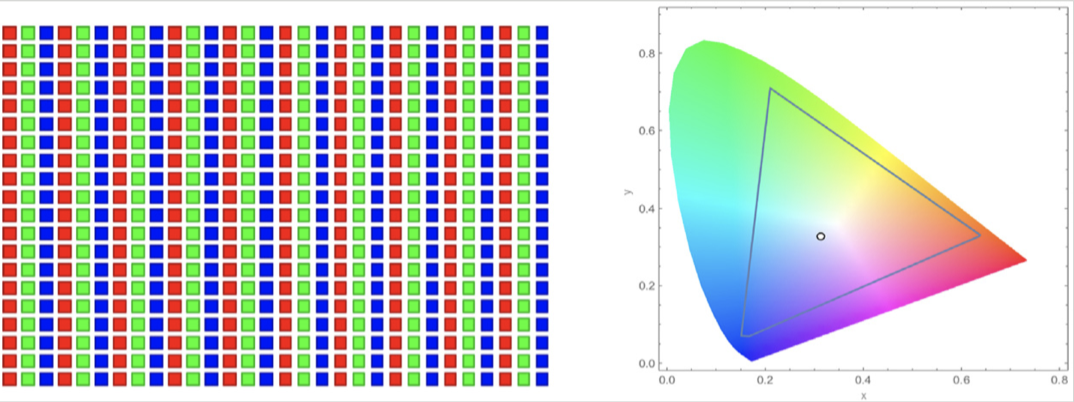
\includegraphics[width=0.9\textwidth]{figs/F2-a1.png}
\end{figure}

这三种颜色的实际允许混合因行业指定的颜色空间而异。 
这里,AdbobeRGB$^{TM}$ 颜色空间中三种颜色的有效组合显示为三角形的内部。 
每个混合的垂直坐标(y 值)和水平坐标(x 值)显示应为 G 和 R 的像素强度分数。像素强度的剩余分数 (1-y-x) 应分配给 B。 
渲染图像时,每个像素的 r、g、b 值用于计算像素的总强度(亮度)以及混合系数(x、y、1-y-x)。
\end{remark}

\begin{figure}[H]
	\centering
	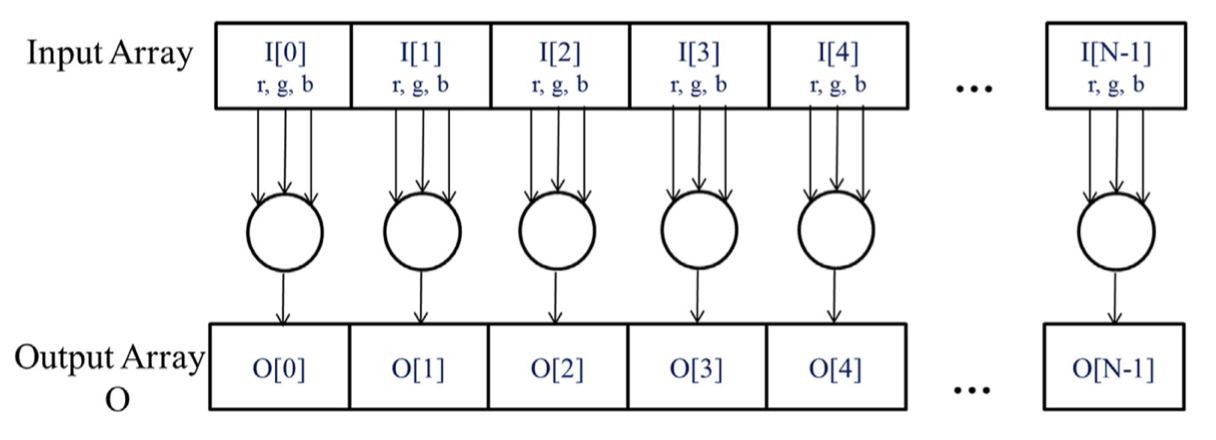
\includegraphics[width=0.9\textwidth]{figs/F2.2.png}
	\caption{\textit{图像到灰度转换中的数据并行性。 像素可以彼此独立地计算。}}
\end{figure}

如果我们将输入视为由 RGB 值数组 I 组织的图像,并将输出视为相应的亮度值数组 O,则我们得到如图 2.2 所示的简单计算结构。 
例如,根据上式计算I[0]中RGB值的加权和,生成O[0]; O[1]是通过计算I[1]中RGB值的加权和生成的; 
O[2]是通过计算I[2]中RGB值的加权和生成的; 等等。 这些每像素计算都不相互依赖。 所有这些都可以独立执行。 
显然,彩色到灰度的转换表现出丰富的数据并行性。 当然,完整应用程序中的数据并行性可能更加复杂,
本书的大部分内容都致力于教授发现和利用数据并行性所必需的并行思维。

\begin{remark}[任务并行与数据并行]
数据并行并不是并行编程中使用的唯一并行类型。 任务并行性也广泛应用于并行编程中。 
任务并行性通常通过应用程序的任务分解来暴露。 例如,一个简单的应用程序可能需要进行向量加法和矩阵向量乘法。 
其中每一个都是一项任务。 如果两个任务可以独立完成,则存在任务并行性。 I/O 和数据传输也是常见的任务源。

在大型应用程序中,通常存在大量独立任务,因此任务并行性也较大。 例如,在分子动力学模拟器中,
自然任务列表包括振动力、旋转力、非键合力的邻居识别、非键合力、速度和位置以及基于速度和位置的其他物理属性。

一般来说,数据并行性是并行程序可扩展性的主要来源。 对于大型数据集,人们通常可以找到丰富的数据并行性,
以便能够利用大规模并行处理器,并允许应用程序性能随着每一代具有更多执行资源的硬件而增长。 
尽管如此,任务并行性也可以在实现性能目标方面发挥重要作用。 稍后在介绍流(stream)时我们将介绍任务并行性。
\end{remark}

\subsection{CUDA C程序结构}
我们现在准备学习如何编写 CUDA C 程序来利用数据并行性来加快执行速度。 
CUDA C\footnote{CUDA C 采用 C++ 特性的趋势一直在稳步推进。 我们将在编程示例中使用其中一些 C++ 特性。} 
以最少的新语法和库函数扩展了流行的 ANSI C 编程语言,
使程序员能够针对包含 CPU 内核和大规模并行 GPU 的异构计算系统。 顾名思义,CUDA C 构建在 NVIDIA 的 CUDA 平台上。 
CUDA是目前最成熟的大规模并行计算框架。 它广泛应用于高性能计算行业,
在最常见的操作系统上提供编译器、调试器和分析器等基本工具。

CUDA C 程序的结构反映了计算机中主机(CPU)和一个或多个设备(GPU)的共存。 
每个 CUDA C 源文件可以混合有主机代码和设备代码。 默认情况下,任何传统 C 程序都是仅包含主机代码的 CUDA 程序。 
人们可以将设备代码添加到任何源文件中。 设备代码清楚地标有特殊的 CUDA C 关键字。 
设备代码包括函数或内核,其代码以数据并行方式执行。

\begin{figure}[H]
	\centering
	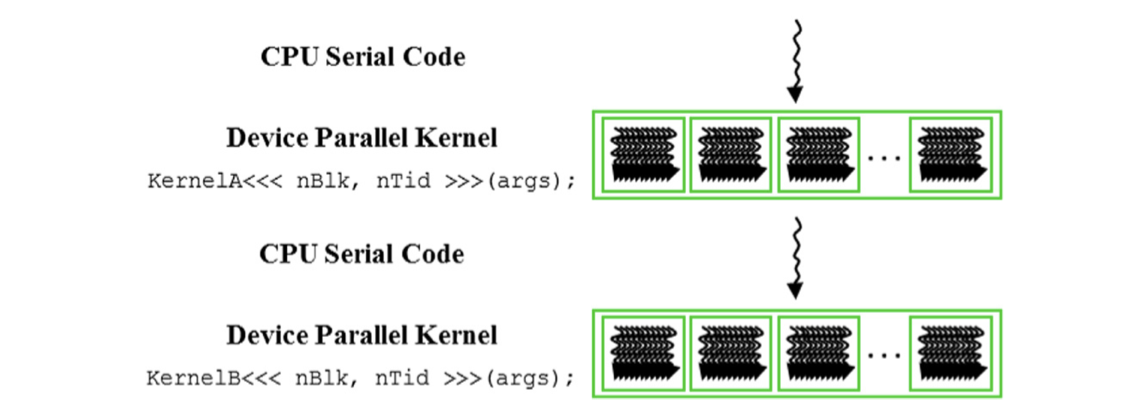
\includegraphics[width=0.9\textwidth]{figs/F2.3.png}
	\caption{\textit{CUDA 程序的执行。}}
\end{figure}

CUDA 程序的执行如图 2.3 所示。 执行从主机代码(CPU 串行代码)开始。 当调用内核函数时,
设备上会启动大量线程来执行内核。 由内核调用启动的所有线程统称为网格。 这些线程是 CUDA 平台中并行执行的主要工具。 
图 2.3 显示了两个线程网格的执行情况。 我们将很快讨论这些网格是如何组织的。 
当网格的所有线程都完成其执行时,网格终止,并且执行在主机上继续,直到启动另一个网格。 
请注意,图 2.3 显示了一个简化模型,其中 CPU 执行和 GPU 执行不重叠。 
许多异构计算应用程序管理重叠的 CPU 和 GPU 执行,以充分利用 CPU 和 GPU。

启动网格通常会生成许多线程来利用数据并行性。 在彩色到灰度转换的示例中,每个线程可用于计算输出数组 O 的一个像素。
在这种情况下,网格启动应生成的线程数等于 图片。 对于大图像,会产生大量线程。 
由于高效的硬件支持,CUDA 程序员可以假设这些线程只需很少的时钟周期即可生成和调度。 
这一假设与传统的 CPU 线程形成对比,传统的 CPU 线程通常需要数千个时钟周期来生成和调度。 
在下一章中,我们将展示如何实现颜色到灰度转换和图像模糊内核。 
在本章的其余部分中,为了简单起见,我们将使用向量加法作为运行示例。

\begin{remark}[线程]
线程是现代计算机中处理器如何执行顺序程序的简化视图。 线程由程序代码、正在执行的代码中的点及其变量和数据结构的值组成。 
就用户而言,线程的执行是顺序的。 人们可以使用源代码级调试器来监视线程的进度,
方法是一次执行一个语句,查看下一个将要执行的语句,并在执行过程中检查变量和数据结构的值。

线程在编程中的应用已经很多年了。 如果程序员想要在应用程序中开始并行执行,他/她可以使用线程库或特殊语言创建和管理多个线程。 
在 CUDA 中,每个线程的执行也是顺序的。 CUDA 程序通过调用内核函数来启动并行执行,
这会导致底层运行时机制启动并行处理数据不同部分的线程网格。
\end{remark}

\subsection{向量加法核函数}
\begin{figure}[H]
	\centering
	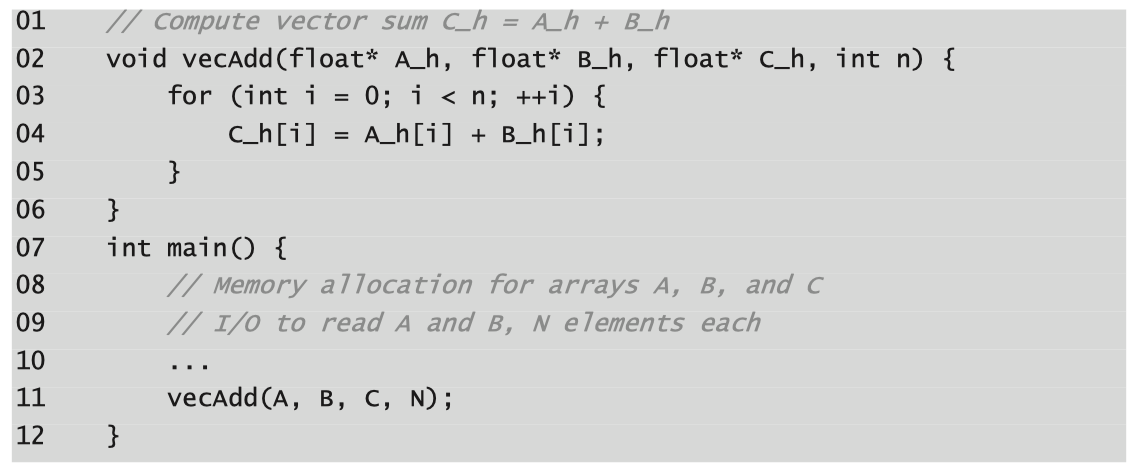
\includegraphics[width=0.9\textwidth]{figs/F2.4.png}
	\caption{\textit{一个简单的传统向量加法 C 代码示例。}}
\end{figure}

我们使用向量加法来演示 CUDA C 程序结构。 向量加法可以说是最简单的数据并行计算——相当于顺序编程中的“Hello World”。 
在我们展示向量加法的内核代码之前,首先回顾一下传统向量加法(主机代码)函数的工作原理会很有帮助。 
图 2.4 显示了一个简单的传统 C 程序,由主函数和向量加法函数组成。 在我们所有的示例中,每当需要区分主机和设备数据时,
我们都会在主机使用的变量名称后添加“\_h”,在设备使用的变量名称后添加“\_d”以 提醒我们自己这些变量的预期用途。 
由于图 2.4 中只有主机代码,因此我们只能看到后缀为“\_h”的变量。

\begin{remark}[C语言中的指针]
	图 2.4 中的函数参数 A、B 和 C 是指针。 在C语言中,可以使用指针来访问变量和数据结构。 浮点变量 V 可以这样声明:
	
float $V$;

指针变量 $P$ 可以这样声明:

float ${ }^{*} P$

通过使用语句 $P=\& V$ 将 $V$ 的地址分配给 $P$,我们使 $P$“指向”$V$。 ${ }^{*} P$ 成为 $V$ 的同义词。 
例如,$U={ }^{*} P$ 将$V$ 的值赋给$U$。 再例如, ${ }^{*} P=3$ 将 $V$ 的值更改为 3 。

$C$ 程序中的数组可以通过指向其 $O^{\text {th }}$ 元素的指针来访问。 
例如,语句 $P=\&(A[0])$ 使 $P$ 指向数组 A 的 $O^{\text {th }}$ 元素。 
P[i] 成为 A[i] 的同义词。 事实上,数组名称 $A$ 本身就是一个指向其 $O^{\text {th }}$ 元素的指针。

在图 2.4 中,将数组名 $A$ 作为函数调用的第一个参数传递给 vecAdd,
使得函数的第一个参数 $A \_h$ 指向 $A$ 的 $0^{\text {th }}$ 元素。 
因此,函数体中的 $A \_h[i]$ 可用于访问主函数中数组 $\mathrm{A}$ 的 $A[i]$。

请参阅 Patt \& Patel(Patt \& Patel,2020),了解 $C$ 中指针的详细用法的简单易懂的解释。
\end{remark}

假设要相加的向量存储在主程序中分配并初始化的数组A和B中。 输出向量位于数组C中,该数组也在主程序中分配。 
为了简洁起见,我们没有显示 A、B 和 C 在主函数中如何分配或初始化的细节。 
指向这些数组的指针连同包含向量长度的变量 N 一起传递给 vecAdd 函数。 
请注意,vecAdd 函数的参数带有“\_h”后缀,以强调它们是由主机使用的。 
当我们在接下来的几个步骤中引入设备代码时,这种命名约定将会很有帮助。

图 2.4 中的 vecAdd 函数使用 for 循环来迭代向量元素。 在第 i 次迭代中,
输出元素 C\_h[i] 接收 A\_h[i] 和 B\_h[i] 的和。 向量长度参数 n 用于控制循环,使迭代次数与向量的长度相匹配。 
该函数分别通过指针A\_h、B\_h和C\_h读取A和B的元素并写入C的元素。 
当vecAdd函数返回时,main函数中的后续语句就可以访问C的新内容。

\begin{figure}[H]
	\centering
	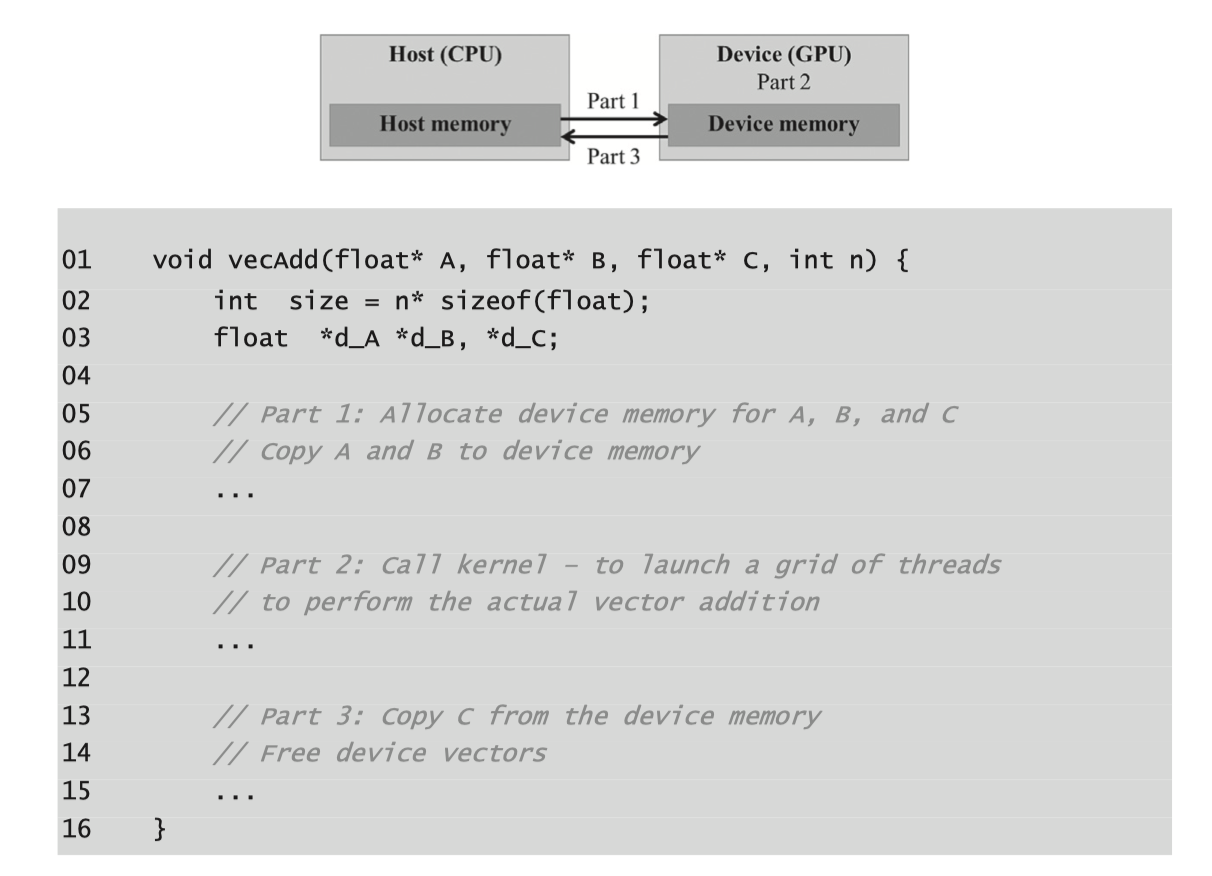
\includegraphics[width=0.9\textwidth]{figs/F2.5.png}
	\caption{\textit{将工作移至设备的修订版 vecAdd 函数的概述。}}
\end{figure}

并行执行向量加法的一种直接方法是修改 vecAdd 函数并将其计算移至设备。 这种修改后的 vecAdd 函数的结构如图 2.5 所示。 
该函数的第 1 部分在设备 (GPU) 内存中分配空间来保存 A、B 和 C 向量的副本,并将 A 和 B 向量从主机内存复制到设备内存。 
第 2 部分调用实际的向量加法内核来启动设备上的线程网格。 
第 3 部分将和向量 C 从设备内存复制到主机内存,并从设备内存中释放三个数组。

请注意,修改后的 vecAdd 函数本质上是一个外包代理,它将输入数据发送到设备,激活设备上的计算,并从设备收集结果。 
代理这样做的方式是主程序甚至不需要知道矢量加法现在实际上是在设备上完成的。 在实践中,这种“透明”的外包模式可能非常低效,
因为所有数据都来回复制。 人们通常会在设备上保留大型且重要的数据结构,并简单地从主机代码中调用它们上的设备功能。 
不过,现在我们将使用简化的透明模型来介绍基本的 CUDA C 程序结构。 
修改后的函数的细节以及内核函数的编写方式将是本章剩余部分的主题。

\subsection{设备全局内存和数据传输}
在当前的 CUDA 系统中,设备通常是硬件卡,带有自己的动态随机存取存储器,称为设备全局存储器,或简称为全局存储器。 
例如,NVIDIA Volta V100 配备 16GB 或 32GB 全局内存。 将其称为“全局”内存,
将其与程序员也可以访问的其他类型的设备内存区分开来。 
有关 CUDA 内存模型和不同类型设备内存的详细信息将在第 5 章“内存架构和数据局部性”中讨论。

对于向量加法内核,在调用内核之前,程序员需要在设备全局内存中分配空间,并将数据从主机内存传输到设备全局内存中分配的空间。 
这对应于图 2.5 的第 1 部分。 类似地,在设备执行之后,程序员需要将结果数据从设备全局存储器传输回主机存储器,
并释放设备全局存储器中不再需要的已分配空间。 这对应于图 2.5 的第 3 部分。 
CUDA运行时系统(通常在主机上运行)提供应用程序编程接口(API)函数来代表程序员执行这些活动。 
从现在开始,我们将简单地说数据从主机传输到设备,作为数据从主机内存复制到设备全局内存的简写。 对于相反的方向也是如此。

图2.5中,vecAdd函数的第1部分和第3部分需要使用CUDA API函数为A、B和C分配设备全局内存; 
将 A 和 B 从主机传输到设备; 向量相加后将 C 从设备传输到主机; 并释放A、B、C的设备全局内存。
我们首先解释内存分配和释放函数。

\begin{figure}[H]
	\centering
	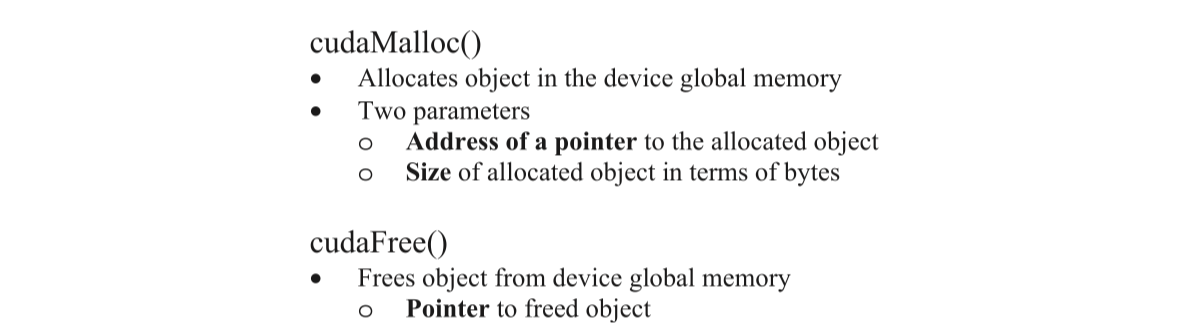
\includegraphics[width=0.9\textwidth]{figs/F2.6.png}
	\caption{\textit{用于管理设备全局内存的 CUDA API 函数。}}
\end{figure}

图 2.6 显示了两个用于分配和释放设备全局内存的 API 函数。 
可以从主机代码调用 cudaMalloc 函数来为对象分配一块设备全局内存。 
读者应该注意到 cudaMalloc 和标准 C 运行时库 malloc 函数之间惊人的相似性。 
这是故意的; CUDA C 是具有最少扩展的 C。 CUDA C使用标准C运行时库malloc函数来管理主机内存
\footnote{CUDA C 还具有更高级的库函数,用于在主机内存中分配空间。 我们将在第 20 章“异构计算集群编程”中讨论它们。} ,
并将cudaMalloc作为C运行时库的扩展添加。 通过使接口尽可能接近原始 C 运行时库,
CUDA C 最大限度地减少了 C 程序员重新学习这些扩展的使用所花费的时间。

cudaMalloc 函数的第一个参数是指针变量的地址,该变量将被设置为指向分配的对象。
指针变量的地址应转换为 (void ** ),因为该函数需要一个通用指针; 内存分配函数是一个通用函数,不限于任何特定类型的对象
\footnote{cudaMalloc 返回通用对象这一事实使得动态分配的多维数组的使用更加复杂。 我们将在 3.2 节中解决这个问题。} 。
该参数允许 cudaMalloc 函数将分配的内存的地址写入提供的指针变量,无论其类型如何
\footnote{请注意,cudaMalloc 的格式与 C malloc 函数不同。 C malloc 函数返回指向已分配对象的指针。 
它只需要一个参数来指定分配对象的大小。 cudaMalloc 函数写入地址作为第一个参数给出的指针变量。 
因此,cudaMalloc 函数有两个参数。 
cudaMalloc 的双参数格式允许它使用返回值以与其他 CUDA API 函数相同的方式报告任何错误。}。
调用内核的主机代码将此指针值传递给需要访问已分配内存对象的内核。 
cudaMalloc 函数的第二个参数给出要分配的数据的大小(以字节数为单位)。 
第二个参数的用法与 C malloc 函数的大小参数一致。

我们现在用下面简单的代码示例来说明cudaMalloc和cudaFree的使用:

float *A\_d 

int size=n * sizeof(float);

cudaMalloc((void ** )\&A\_d, size);

... cudaFree(A\_d);

这是图 2.5 中示例的延续。 为了清楚起见,我们在指针变量后面加上“\_d”后缀,以指示它指向设备全局内存中的对象。 
传递给 cudaMalloc 的第一个参数是转换为 void 指针的指针 A\_d(即 \&A\_d)的地址。 
当cudaMalloc返回时,A\_d将指向为A向量分配的设备全局内存区域。 传递给 cudaMalloc 的第二个参数是要分配的区域的大小。 
由于 size 是以字节数为单位的,因此程序员在确定 size 的值时需要将数组中的元素数转换为字节数。 
例如,在为包含 n 个单精度浮点元素的数组分配空间时,size 的值将是单精度浮点数大小的 n 倍,在当今的计算机中为 4 个字节。 
因此,size 的值将为 n × 4。计算后,以指针 A\_d 作为参数调用 cudaFree,以从设备全局内存中释放 A 向量的存储空间。 
注意cudaFree不需要改变A\_d的值; 它只需要使用A\_d的值将分配的内存返回到可用池。 
因此,只有 A\_d 的值而不是地址作为参数传递。

A\_d、B\_d 和 C\_d 中的地址指向设备全局内存中的位置。 这些地址不应在主机代码中取消引用。 
它们应该用于调用API函数和内核函数。 在主机代码中取消引用设备全局内存指针可能会导致异常或其他类型的运行时错误。

读者应该使用类似的 B\_d 和 C\_d 指针变量声明及其相应的 cudaMalloc 调用来完成图 2.5 中 vecAdd 示例的第 1 部分。 
此外,图 2.5 中的第 3 部分可以通过调用 B\_d 和 C\_d 的 cudaFree 来完成。

\begin{figure}[H]
	\centering
	
\includegraphics[width=0.9\textwidth]{figs/F2.7.png}
	\caption{\textit{CUDA API 函数用于主机和设备之间的数据传输。}}
\end{figure}

一旦主机代码在设备全局存储器中为数据对象分配了空间,它就可以请求将数据从主机传输到设备。 
这是通过调用 CUDA API 函数之一来完成的。 图 2.7 显示了这样一个 API 函数 cudaMemcpy。 
cudaMemcpy 函数有四个参数。 第一个参数是指向要复制的数据对象的目标位置的指针。 第二个参数指向源位置。 
第三个参数指定要复制的字节数。 第四个参数表示复制涉及的内存类型:从主机到主机、从主机到设备、从设备到主机、从设备到设备。 
例如,存储器复制功能可用于将数据从设备全局存储器中的一个位置复制到设备全局存储器中的另一位置。

vecAdd 函数调用 cudaMemcpy 函数,在相加之前将 A\_h 和 B\_h 向量从主机内存复制到设备内存中的 A\_d 和 B\_d,
并在相加完成后将 C\_d 向量从设备内存复制到主机内存中的 C\_h 完毕。 
假设 A\_h、B\_h、A\_d、B\_d 和 size 的值已经按照我们之前讨论的那样设置,则三个 cudaMemcpy 调用如下所示。 
两个符号常量 cudaMemcpyHostToDevice 和 cudaMemcpyDeviceToHost 是 CUDA 编程环境可识别的预定义常量。 
请注意,通过正确排序源指针和目标指针并使用适合传输类型的常量,可以使用同一函数在两个方向上传输数据。

cudaMemcpy(A\_d, A\_h, size, cudaMemcpyHostToDevice); 

cudaMemcpy(B\_d, B\_h, size, cudaMemcpyHostToDevice); 

...

cudaMemcpy(C\_h, C\_d, size, cudaMemcpyDeviceToHost);

总而言之,图2.4中的主程序调用vecAdd,它也在主机上执行。 vecAdd 函数如图 2.5 所示,在设备全局内存中分配空间,
请求数据传输,并调用执行实际向量加法的内核。 我们将这种类型的主机代码称为调用内核的存根。 
我们在图 2.8 中展示了 vecAdd 函数的更完整版本。

\begin{figure}[H]
	\centering
	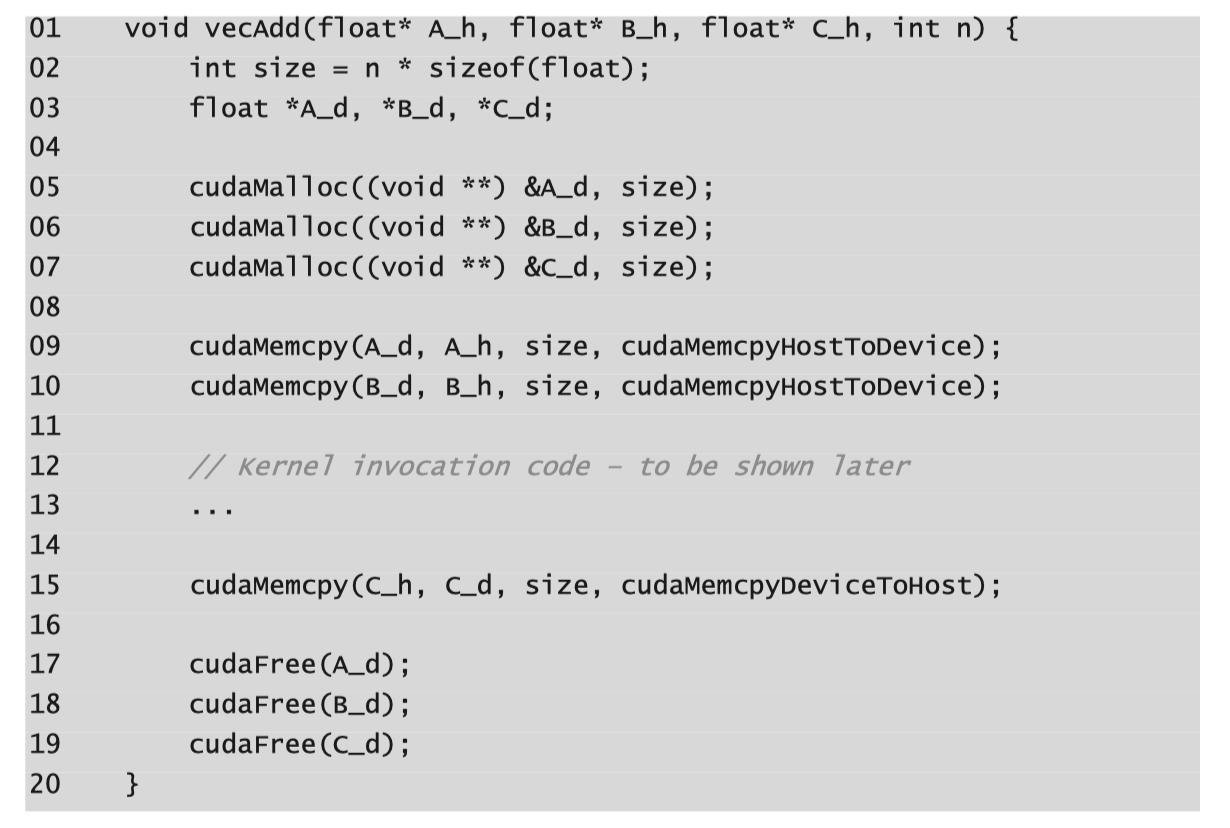
\includegraphics[width=0.9\textwidth]{figs/F2.8.png}
	\caption{\textit{vecAdd() 的更完整版本。}}
\end{figure}

与图2.5相比,图2.8中的vecAdd函数对于第1部分和第3部分来说是完整的。第1部分为A\_d、B\_d和C\_d分配设备全局内存,
并将A\_h传输到A\_d,将B\_h传输到B\_d。 这是通过调用 cudaMalloc 和 cudaMemcpy 来完成的功能。 
鼓励读者使用适当的参数值编写自己的函数调用,并将他们的代码与图 2.8 所示的代码进行比较。 
第 2 部分调用内核,并将在下面的小节中描述。 第 3 部分将向量和数据从设备复制到主机,以便这些值在主函数中可用。 
这是通过调用 cudaMemcpy 函数来完成的。 然后,它从设备全局内存中释放 A\_d、B\_d 和 C\_d 的内存,
这是通过调用 cudaFree 函数来完成的(图 2.9)。

\begin{remark}[CUDA 中的错误检查和处理]
	一般来说,检查和处理错误对于程序来说很重要。 CUDA API 函数返回标志,指示它们在处理请求时是否发生错误。 
	大多数错误是由于调用中使用的参数值不正确造成的。
	
为简洁起见,我们不会在示例中显示错误检查代码。 例如,图 2.9 显示了对 cudaMalloc 的调用:

cudaMalloc((void $\left.{ }^{* *}\right) \& A \_d$, size $)$;

在实践中,我们应该用测试错误条件的代码包围调用并打印出错误消息,以便用户可以知道发生了错误。 此类检查代码的简单版本如下:

cudaError\_t err = cudaMalloc((void**) \&A\_d, size);

if (error != cudaSuccess) \{

	printf(“\%s in \%s at line \%d \textbackslash n”, 
	        cudaGetErrorString(err), \_\_FILE\_\_, \_\_LINE\_\_);

	exit(EXIT\_FAILURE); 

\}

这样,如果系统的设备内存不足,用户将收到有关情况的通知。 这可以节省许多小时的调试时间。

可以定义一个 $C$ 宏来使源代码中的检查代码更加简洁。
\end{remark}

\subsection{核函数与线程}
我们现在准备更多地讨论 CUDA C 内核函数以及调用这些内核函数的效果。 在 CUDA C 中,
内核函数指定在并行阶段由所有线程执行的代码。 由于所有这些线程都执行相同的代码,
因此 CUDA C 编程是著名的单程序多数据 (SPMD)(Atallah,1998)并行编程风格的一个实例,
这是并行计算系统的一种流行编程风格\footnote{请注意,SPMD 与 SIMD(单指令多数据)不同 [Flynn 1972]。 
在 SPMD 系统中,并行处理单元对数据的多个部分执行相同的程序。 然而,这些处理单元不需要同时执行相同的指令。 
在 SIMD 系统中,所有处理单元在任何时刻都执行相同的指令。} 。

当程序的主机代码调用内核时,CUDA 运行时系统会启动组织成两级层次结构的线程网格。 每个网格都组织为线程块数组,
为简洁起见,我们将其称为块。 网格中的所有块的大小相同; 在当前系统上,每个块最多可以包含 1024 个线程
\footnote{在 CUDA 3.0 及更高版本中,每个线程块最多可以有 1024 个线程。 
一些早期的 CUDA 版本仅允许块中最多 512 个线程。} 。 
图 2.9 显示了一个示例,其中每个块由 256 个线程组成。 
每个线程都由一个来自方框的卷曲箭头表示,该方框标有块中线程的索引号。

\begin{figure}[H]
	\centering
	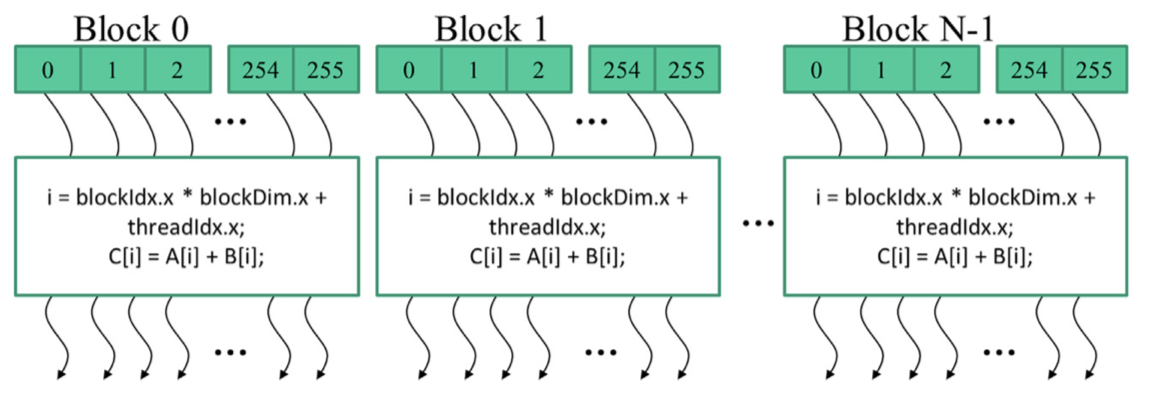
\includegraphics[width=0.9\textwidth]{figs/F2.9.png}
	\caption{\textit{网格中的所有线程都执行相同的内核代码。}}
\end{figure}

\begin{remark}[内置变量]
	许多编程语言都有内置变量。 这些变量具有特殊的含义和目的。 
	这些变量的值通常由运行时系统预先初始化,并且在程序中通常是只读的。 程序员应避免出于任何其他目的重新定义这些变量。
\end{remark}

每个线程块中的线程总数由调用内核时的主机代码指定。 可以在主机代码的不同部分使用不同数量的线程来调用相同的内核。 
对于给定的线程网格,块中的线程数可在名为 blockDim 的内置变量中获得。 
blockDim 变量是一个具有三个无符号整数字段(x、y 和 z)的结构,可帮助程序员将线程组织成一维、二维或三维数组。 
对于一维组织,仅使用 x 字段。 对于二维组织,使用 x 和 y 字段。 对于三维结构,使用所有三个 x、y 和 z 字段。 
组织线程的维度选择通常反映了数据的维度。 这是有道理的,因为创建线程是为了并行处理数据,
因此线程的组织很自然地反映了数据的组织。 在图2.9中,每个线程块被组织为一维线程数组,因为数据是一维向量。 
blockDim.x变量的值表示每个块中的线程总数,在图2.9中为256。 
一般来说,出于硬件效率的考虑,建议线程块每个维度的线程数量为32的倍数。 我们稍后会再讨论这个问题。

CUDA 内核可以访问另外两个内置变量(threadIdx 和 blockIdx),
这些变量允许线程彼此区分并确定每个线程要处理的数据区域。 threadIdx 变量为每个线程提供块内的唯一坐标。 
在图2.9中,由于我们使用一维线程组织,因此仅使用threadIdx.x。 
每个线程的 threadIdx.x 值显示在图 2.9 中每个线程的小阴影框中。 每个块中的第一个线程的 threadIdx.x 变量的值为 0,
第二个线程的值为 1,第三个线程的值为 2,依此类推。

\begin{remark}[层级组织]
与 CUDA 线程一样,许多现实世界的系统都是分层组织的。 美国的电话系统就是一个很好的例子。 
在顶层,电话系统由“区域”组成,每个区域对应一个地理区域。 同一区域内的所有电话线路都具有相同的 3 位数“区号”。 
电话区有时比城市还要大。 例如,伊利诺伊州中部的许多县市都在同一个电话区域内,并且共享相同的区号217。
在一个区域内,每条电话线都有一个七位数字的本地电话号码,这使得每个区域最多可以拥有约 一千万个数字。

可以将每条电话线视为一个 CUDA 线程,其中 blockIdx 的值为区号,threadIdx 的值为七位本地号码。 
这种分层组织允许系统拥有大量电话线路,同时保留呼叫同一区域的“局部性”。 
即拨打同一地区的电话线路时,只需拨打本地号码即可。 只要我们大部分的电话都是在本地拨打,很少需要拨打区号。 
如果我们偶尔需要拨打另一个地区的电话线,我们拨打 1 和区号,然后拨打本地号码。 
(这就是为什么任何区域中的本地编号都不应以 1 开头的原因。)CUDA 线程的分层组织还提供了一种局部性形式。 
我们很快就会研究这个地方。
\end{remark}

blockIdx 变量为块中的所有线程提供一个公共块坐标。 在图 2.9 中,第一个块中的所有线程的 blockIdx.x 变量的值为 0,
第二个线程块中的所有线程的值为 1,依此类推。 与电话系统进行类比,我们可以将 threadIdx.x 视为本地电话号码,
将 blockIdx.x 视为区号。 两者共同为全国的每条电话线提供了唯一的电话号码。 
类似地,每个线程可以组合其 threadIdx 和 blockIdx 值,在整个网格中为自己创建唯一的全局索引。

在图 2.9 中,唯一的全局索引 i 的计算公式为 i=blockIdx.x × blockDim.x + ThreadIdx.x。 
回想一下,在我们的示例中,blockDim 是 256。 块 0 中线程的 i 值范围是 0 到 255。 
块 1 中线程的 i 值范围是 256 到 511。 块 2 中线程的 i 值范围是 512 到 767。 
这三个块中的线程形成了从 0 到 767 的值的连续覆盖。由于每个线程使用 i 访问 A、B 和 C,
因此这些线程覆盖了原始循环的前 768 次迭代。 通过启动具有更多块的网格,可以处理更大的向量。 
通过启动具有 n 个或更多线程的网格,可以处理长度为 n 的向量。

\begin{figure}[H]
	\centering
	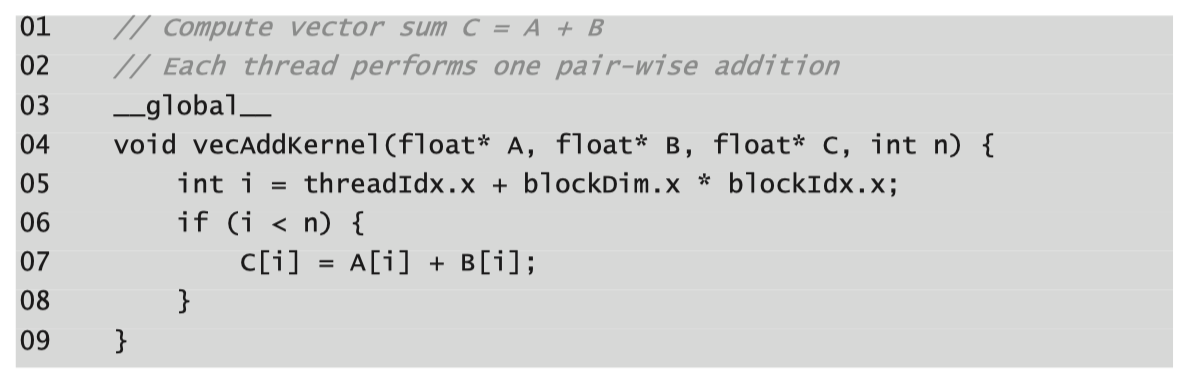
\includegraphics[width=0.9\textwidth]{figs/F2.10.png}
	\caption{\textit{向量加法核函数。}}
\end{figure}

图 2.10 显示了向量加法的核函数。 请注意,我们不在内核中使用“\_h”和“\_d”约定,因为不存在潜在的混淆。 
在我们的示例中,我们将无法访问主机内存。 内核的语法是 ANSI C,并带有一些值得注意的扩展。 
首先,在 vecAddKernel 函数的声明前面有一个 CUDA-C 特定关键字“\_\_global\_\_”。 
该关键字指示该函数是一个内核,并且可以调用它来在设备上生成线程网格。

\begin{figure}[H]
	\centering
	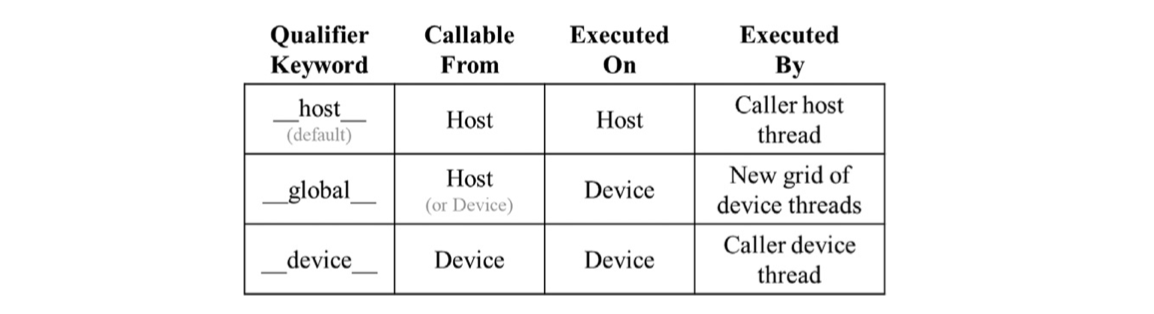
\includegraphics[width=0.9\textwidth]{figs/F2.11.png}
	\caption{\textit{用于函数声明的 CUDA C 关键字。}}
\end{figure}

一般来说,CUDA C 使用三个可在函数声明中使用的限定符关键字扩展了 C 语言。 
这些关键字的含义总结在图 2.11 中。 “\_\_global\_\_”关键字表示所声明的函数是 CUDA C 内核函数。 
请注意,“global”一词的两侧各有两个下划线字符。 这样的内核函数在设备上执行并且可以从主机调用。 
在支持动态并行的 CUDA 系统中,也可以从设备调用它,我们将在第 21 章“CUDA 动态并行”中看到。 
重要的特征是调用这样的内核函数会导致在设备上启动新的线程网格。

“\_\_device\_\_”关键字表示所声明的函数是 CUDA 设备函数。 设备函数在 CUDA 设备上执行,
并且只能从内核函数或其他设备函数调用。 设备函数由调用它的设备线程执行,不会导致启动任何新的设备线程
\footnote{稍后我们将解释不同代 CUDA 中使用间接函数调用和递归的规则。 
一般来说,应该避免在其设备函数和内核函数中使用递归和间接函数调用,以实现最大的可移植性。} 。

“\_\_host\_\_”关键字表示所声明的函数是 CUDA 主机函数。 主机函数只是在主机上执行的传统 C 函数,
并且只能从另一个主机函数调用。 默认情况下,如果 CUDA 程序中的所有函数在其声明中没有任何 CUDA 关键字,
则它们都是主机函数。 这是有道理的,因为许多 CUDA 应用程序都是从纯 CPU 执行环境移植的。 
程序员在移植过程中会添加内核函数和设备函数。 原始功能仍作为主机功能。 
将所有函数默认为主机函数可以使程序员免去更改所有原始函数声明的繁琐工作。

请注意,可以在函数声明中同时使用“\_\_host\_\_”和“\_\_device\_\_”。 
这种组合告诉编译系统为同一函数生成两个版本的目标代码。 一种是在主机上执行的,并且只能从主机函数中调用。 
另一个在设备上执行,只能从设备或内核函数中调用。 当可以重新编译相同的函数源代码以生成设备版本时,这支持常见的用例。 
许多用户库函数可能属于这一类。

C 的第二个值得注意的扩展,如图 2.10 所示,是内置变量“threadIdx”, “blockIdx”和“blockDim”。 
回想一下,所有线程都执行相同的内核代码,并且需要有一种方法让它们彼此区分并将每个线程引导至数据的特定部分。 
这些内置变量是线程访问为线程提供识别坐标的硬件寄存器的方法。 
不同的线程将在其 threadIdx.x, blockIdx.x 和 blockDim.x 变量中看到不同的值。 
为了便于阅读,我们有时会在讨论中将线程称为线程 blockIdx.x, threadIdx.x。

图 2.10 中有一个自动(局部)变量 i。 在 CUDA 内核函数中,自动变量是每个线程私有的。 
也就是说,将为每个线程生成一个 i 版本。 如果网格以 10,000 个线程启动,则 i 将会有 10,000 个版本,每个线程一个。 
线程为其 i 变量分配的值对其他线程不可见。 我们将在第 5 章“内存架构和数据局部性”中更详细地讨论这些自动变量。

快速比较图 2.4 和图 2.10 揭示了对 CUDA 内核的重要见解。 图 2.10 中的核函数没有与图 2.4 中的循环相对应的循环。 
读者应该问循环去了哪里。 答案是循环现在被线程网格所取代。 整个网格相当于循环。 网格中的每个线程对应于原始循环的一次迭代。 
这有时称为循环并行,其中原始顺序代码的迭代由线程并行执行。

注意图 2.10 中的 addVecKernel 中有一个 if(i < n) 语句。 这是因为并非所有向量长度都可以表示为块大小的倍数。 
例如,假设向量长度为 100。最小有效线程块维度为 32。假设我们选择 32 作为块大小。 
需要启动 4 个线程块来处理所有 100 个向量元素。 然而,四个线程块将有 128 个线程。 
我们需要禁止线程块 3 中的最后 28 个线程执行原始程序未预期的工作。 由于所有线程都将执行相同的代码,
因此所有线程都将根据 n(即 100)测试其 i 值。使用 if (i , n) 语句,前 100 个线程将执行加法,而最后 28 个则不会。 
这允许调用内核来处理任意长度的向量。

\subsection{调用核函数}
\begin{figure}[H]
	\centering
	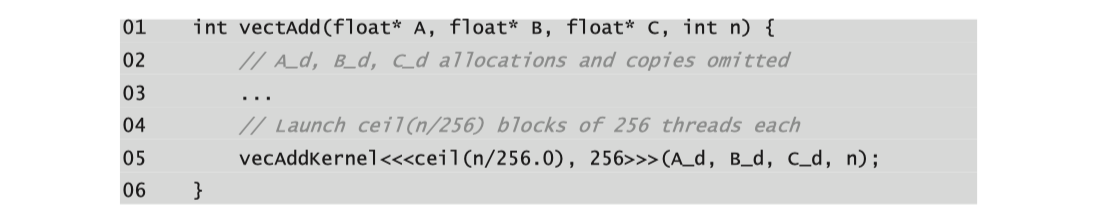
\includegraphics[width=0.9\textwidth]{figs/F2.12.png}
	\caption{\textit{向量加法内核调用语句。}}
\end{figure}

实现内核函数后,剩下的步骤是从主机代码调用该函数来启动网格。 如图 2.12 所示。 当主机代码调用内核时,
它通过执行配置参数设置网格和线程块尺寸。 配置参数在传统 C 函数参数之前的“$<<<$”和“$>>>$”之间给出。 
第一个配置参数给出了网格中的块数。 第二个指定每个块中的线程数。 在此示例中,每个块中有 256 个线程。 
为了确保网格中有足够的线程来覆盖所有向量元素,
我们需要将网格中的块数设置为所需线程数的上限除法(将商四舍五入到直接较高的整数值) 
(本例中为 n)乘以线程块大小(本例中为 256)。 有多种方法可以进行上界划分。 一种方法是将 C 上限函数应用于 n/256.0。 
使用浮点值 256.0 确保我们为除法生成一个浮点值,以便上限值函数可以正确地将其向上舍入。 例如,如果我们想要 1000 个线程,
我们将启动 $ceil(1000/256.0) = 4$ 个线程块。 结果,该语句将启动 $4 \times 256 = 1024$ 个线程。 
通过内核中的 if(i < n) 语句,如图 2.10 所示,前 1000 个线程将对 1000 个向量元素执行加法。 其余 24 个不会。

\begin{figure}[H]
	\centering
	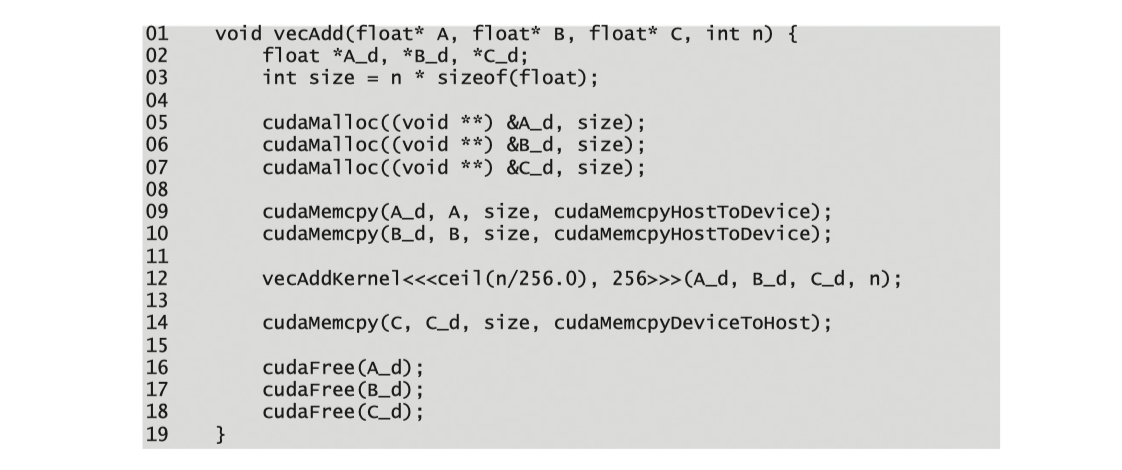
\includegraphics[width=0.9\textwidth]{figs/F2.13.png}
	\caption{\textit{vecAdd 函数中主机代码的完整版本。}}
\end{figure}

图 2.13 显示了 vecAdd 函数中的最终主机代码。 该源代码完成了图 2.5 中的框架。 
2.12和2.13共同说明了一个简单的CUDA程序,它由主机代码和设备内核组成。 该代码被硬连线为使用每个 256 个线程的线程块
\footnote{虽然我们在此示例中使用任意块大小 256,但块大小应由稍后将介绍的许多因素确定。} 。 
但是,所使用的线程块的数量取决于向量 (n) 的长度。 如果n为750,则将使用三个线程块。 如果n为4000,则将使用16个线程块。 
如果n为2,000,000,则将使用7813个块。 请注意,所有线程块都对向量的不同部分进行操作。 
它们可以按任意顺序执行。 程序员不得对执行顺序做出任何假设。 
具有少量执行资源的小型 GPU 可能仅并行执行这些线程块中的一个或两个。 更大的 GPU 可以并行执行 64 或 128 个块。 
这使得 CUDA 内核在硬件执行速度方面具有可扩展性。 
也就是说,相同的代码在小型 GPU 上以较低的速度运行,而在较大的 GPU 上以较高的速度运行。 
我们将在第 4 章“计算架构和调度”中重新讨论这一点。

需要再次指出的是,使用向量加法示例是为了简单起见。 
实际上,分配设备内存、从主机到设备的输入数据传输、
从设备到主机的输出数据传输以及取消分配设备内存的开销可能会使生成的代码比图 2.4 中的原始顺序代码慢。 
这是因为内核完成的计算量相对于处理或传输的数据量来说很小。 对于两个浮点输入操作数和一个浮点输出操作数仅执行一次加法。 
实际应用程序通常具有相对于处理的数据量而言需要更多工作的内核,这使得额外的开销是值得的。 
实际应用程序还倾向于在多个内核调用之间将数据保留在设备内存中,以便可以分摊开销。 我们将展示此类应用的几个示例。

\subsection{编译}
我们已经看到,实现 CUDA C 内核需要使用各种不属于 C 的扩展。一旦在代码中使用了这些扩展,传统的 C 编译器就不再可接受。 
代码需要由能够识别和理解这些扩展的编译器来编译,例如 NVCC(NVIDIA C 编译器)。 
如图2.14顶部所示,NVCC编译器处理CUDA C程序,使用CUDA关键字来分离主机代码和设备代码。 
主机代码是直接的 ANSI C 代码,使用主机的标准 C/C++ 编译器进行编译,并作为传统 CPU 进程运行。 
设备代码标有 CUDA 关键字,指定 CUDA 内核及其关联的辅助函数和数据结构,由 NVCC 编译成称为 PTX 文件的虚拟二进制文件。 
这些 PTX 文件由 NVCC 的运行时组件进一步编译为真实对象文件,并在支持 CUDA 的 GPU 设备上执行。

\begin{figure}[H]
	\centering
	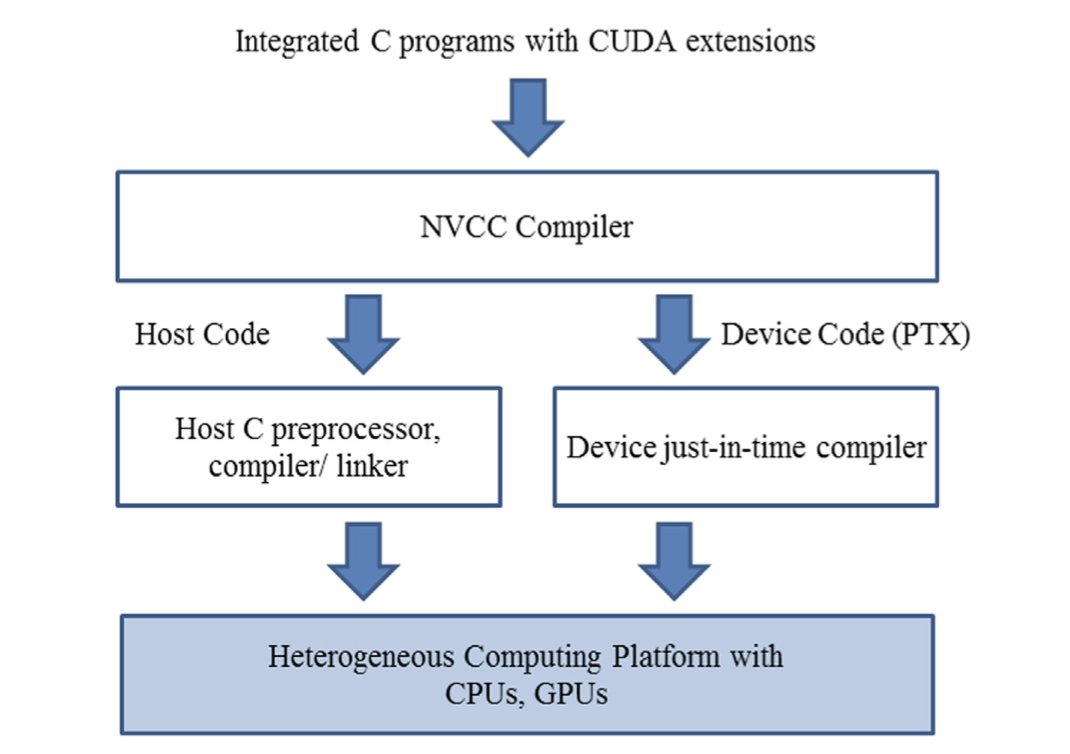
\includegraphics[width=0.9\textwidth]{figs/F2.14.png}
	\caption{\textit{CUDA C 程序的编译过程概述。}}
\end{figure}

\subsection{总结}
本章提供了 CUDA C 编程模型的快速、简化的概述。 CUDA C 扩展了 C 语言以支持并行计算。 
我们在本章中讨论了这些扩展的一个重要子集。 为了您的方便,我们将本章讨论的扩展总结如下:

\subsubsection{函数声明}
CUDA C 扩展了 C 函数声明语法以支持异构并行计算。 图 2.12 总结了这些扩展。 
使用“\_\_global\_\_”、“\_\_device\_\_”或“\_\_host\_\_”之一,
CUDA C 程序员可以指示编译器生成内核函数、设备函数或主机函数。 所有不带任何这些关键字的函数声明都默认为宿主函数。 
如果在函数声明中同时使用“\_\_host\_\_”和“\_\_device\_\_”,编译器会生成该函数的两个版本,
一种用于设备,一种用于主机。 如果函数声明没有任何 CUDA C 扩展关键字,则该函数默认为主机函数。

\subsubsection{核函数调用和网格启动}
CUDA C 使用 $<<<$ 和 $>>>$ 包围的内核执行配置参数扩展了 C 函数调用语法。
这些执行配置参数仅在调用内核函数来启动网格时使用。 
我们讨论了定义网格尺寸和每个块尺寸的执行配置参数。 读者应参阅 CUDA 编程指南(NVIDIA,2021),
了解内核启动扩展以及其他类型的执行配置参数的更多详细信息。


\subsubsection{内置变量}
CUDA 内核可以访问一组内置的、预定义的只读变量,这些变量允许每个线程将自己与其他线程区分开来,并确定要处理的数据区域。 
我们在本章中讨论了 threadIdx、blockDim 和 blockIdx 变量。 
在第 3 章“多维网格和数据”中,我们将讨论使用这些变量的更多细节。

CUDA支持一组API函数来为CUDA C程序提供服务。 我们在本章中讨论的服务是 cudaMalloc、cudaFree 和 cudaMemcpy 函数。 
这些函数由主机代码调用,以分别代表调用程序分配设备全局内存、释放设备全局内存以及在主机和设备之间传输数据。 
读者可参考《CUDA C 编程指南》了解其他 CUDA API 函数。


\subsubsection{运行时应用程序编程接口}
本章的目标是介绍 CUDA C 的核心概念以及用于编写简单的 CUDA C 程序的基本 CUDA C 扩展。 
本章绝不是对所有 CUDA 功能的全面介绍。 其中一些功能将在本书的其余部分中介绍。 
然而,我们的重点将放在这些功能支持的关键并行计算概念上。 我们将仅介绍并行编程技术的代码示例中所需的 CUDA C 功能。 
一般来说,我们鼓励读者始终查阅 CUDA C 编程指南,以了解 CUDA C 功能的更多详细信息。